\documentclass[12pt,letterpaper]{article}
\usepackage{fullpage}
\usepackage[top=2cm, bottom=4.5cm, left=2.5cm, right=2.5cm]{geometry}
\usepackage{amsmath,amsthm,amsfonts,amssymb,amscd}
\usepackage{lastpage}
\usepackage{enumerate}
\usepackage{fancyhdr}
\usepackage{mathrsfs}
\usepackage{xcolor}
\usepackage{graphicx}
\usepackage{listings}
\usepackage{hyperref}
\usepackage{tikz}
\usepackage{relsize}
\usepackage{fancyvrb}
\usepackage{import}
\usetikzlibrary{shapes.geometric,fit}

\hypersetup{%
  colorlinks=true,
  linkcolor=blue,
  linkbordercolor={0 0 1}
}

\setlength{\parindent}{0.0in}
\setlength{\parskip}{0.05in}

\theoremstyle{definition}
\newtheorem*{statement}{Statement}
\newtheorem*{claim}{Claim}
\newtheorem*{theorem}{Theorem}
\newtheorem*{lemma}{Lemma}

\newcommand{\contra}{\Rightarrow\!\Leftarrow}
\newcommand{\R}{\mathbb{R}}
\newcommand{\F}{\mathbb{F}}
\newcommand{\Z}{\mathbb{Z}}
\newcommand{\Zeq}{\mathbb{Z}_{\geq 0}}
\newcommand{\Zg}{\mathbb{Z}_{>0}}
\newcommand{\Req}{\mathbb{R}_{\geq 0}}
\newcommand{\Rg}{\mathbb{R}_{>0}}
\newcommand{\N}{\mathbb{N}}
\newcommand{\Q}{\mathbb{Q}}
\newcommand{\C}{\mathbb{C}}
\DeclareMathOperator{\Cov}{Cov}
\DeclareMathOperator{\Var}{Var}

\newcommand{\incfig}[1] {%
    % \def\svgwidth{\columnwidth}
    \import{./figures/}{#1.pdf_tex}
}

\title{ECON 3412 HW 1}
\author{David Chen, dc3451}

\begin{document}

\maketitle
% \today

\section*{Problem 1}

\subsection*{a}

The sample means are
\begin{align*}
  \overline{X} &= \frac{1}{n}\sum X_{i} = \frac{1}{6}(1016.6+1089.9 +827.7+1021.3+1493.3 +720.1) = 1028.15 \\
  \overline{Y} &= \frac{1}{n}\sum Y_{i} = \frac{1}{6}(320.0+448.4+575.4+219.5+561.3+195.7) = 386.72
\end{align*}

\subsection*{b}

I assume by $s_{X}, s_{Y}$ that the sample standard deviation is wanted. (All the subsequent parts, when relevant, are computed as the sample covariance, sample correlation, etc.)

\begin{align*}
  s_{X} &= \sqrt{\frac{1}{n-1}\sum (X_{i} - \overline{X})^{2}} = \sqrt{\frac{1}{5}\sum(X_{i} - 1028.15)^{2}} = 266.62 \\
  s_{Y} &= \sqrt{\frac{1}{n-1}\sum (Y_{i} - \overline{Y})^{2}} = \sqrt{\frac{1}{5}\sum(Y_{i} - 386.72)^{2}} = 166.60 \\
\end{align*}

\subsection*{c}

The covariance is given by

\[
  s_{XY} = \frac{1}{n-1}\sum(X_{i} - \overline{X})(Y_{i} - \overline{Y}) = \frac{1}{5}\sum (X - 1028.15)(Y - 386.72) = 21590.7
\]

\subsection*{d}

The sample correlation is given by
\[
  r_{XY} = \frac{s_{XY}}{s_{X}s_{Y}} = \frac{21590.7}{266.62 \cdot 166.60} = 0.486
\]

\subsection*{e}

We have that
\[
  \widehat{\beta_{1}} = \frac{s_{XY}}{s^{2}_{X}} = \frac{21590.7}{266.62^{2}} = 0.3037
\]

\subsection*{f}

\[
  \widehat{\beta_{0}} = \overline{Y} - \widehat{\beta_{1}}\overline{X} = 386.72 - (0.3037)1028.15 = 74.44
\]
\subsection*{g}

We have that each $\widehat{Y_{i}} = 74.44 +  0.3037X_{i}$, so

\begin{center}
  \begin{tabular}{c|c}
    $\widehat{Y_{1}}$ & 383.18 \\ \hline
    $\widehat{Y_{2}}$ & 405.44 \\ \hline
    $\widehat{Y_{3}}$ & 325.81 \\ \hline
    $\widehat{Y_{4}}$ & 384.61 \\ \hline
    $\widehat{Y_{5}}$ & 527.96 \\ \hline
    $\widehat{Y_{6}}$ & 293.13 \\
  \end{tabular}
\end{center}


\subsection*{h}

We have that each $\widehat{u_{i}} = Y_{i} - \widehat{Y_{i}}$, so

\begin{center}
  \begin{tabular}{c|c}
    $\widehat{u_{1}}$ & 63.18 \\ \hline
    $\widehat{u_{2}}$ & -42.96 \\ \hline
    $\widehat{u_{3}}$ & -249.59 \\ \hline
    $\widehat{u_{4}}$ & 165.11 \\ \hline
    $\widehat{u_{5}}$ & -33.34 \\ \hline
    $\widehat{u_{6}}$ & 97.43 \\
  \end{tabular}
\end{center}

\section*{Problem 2}

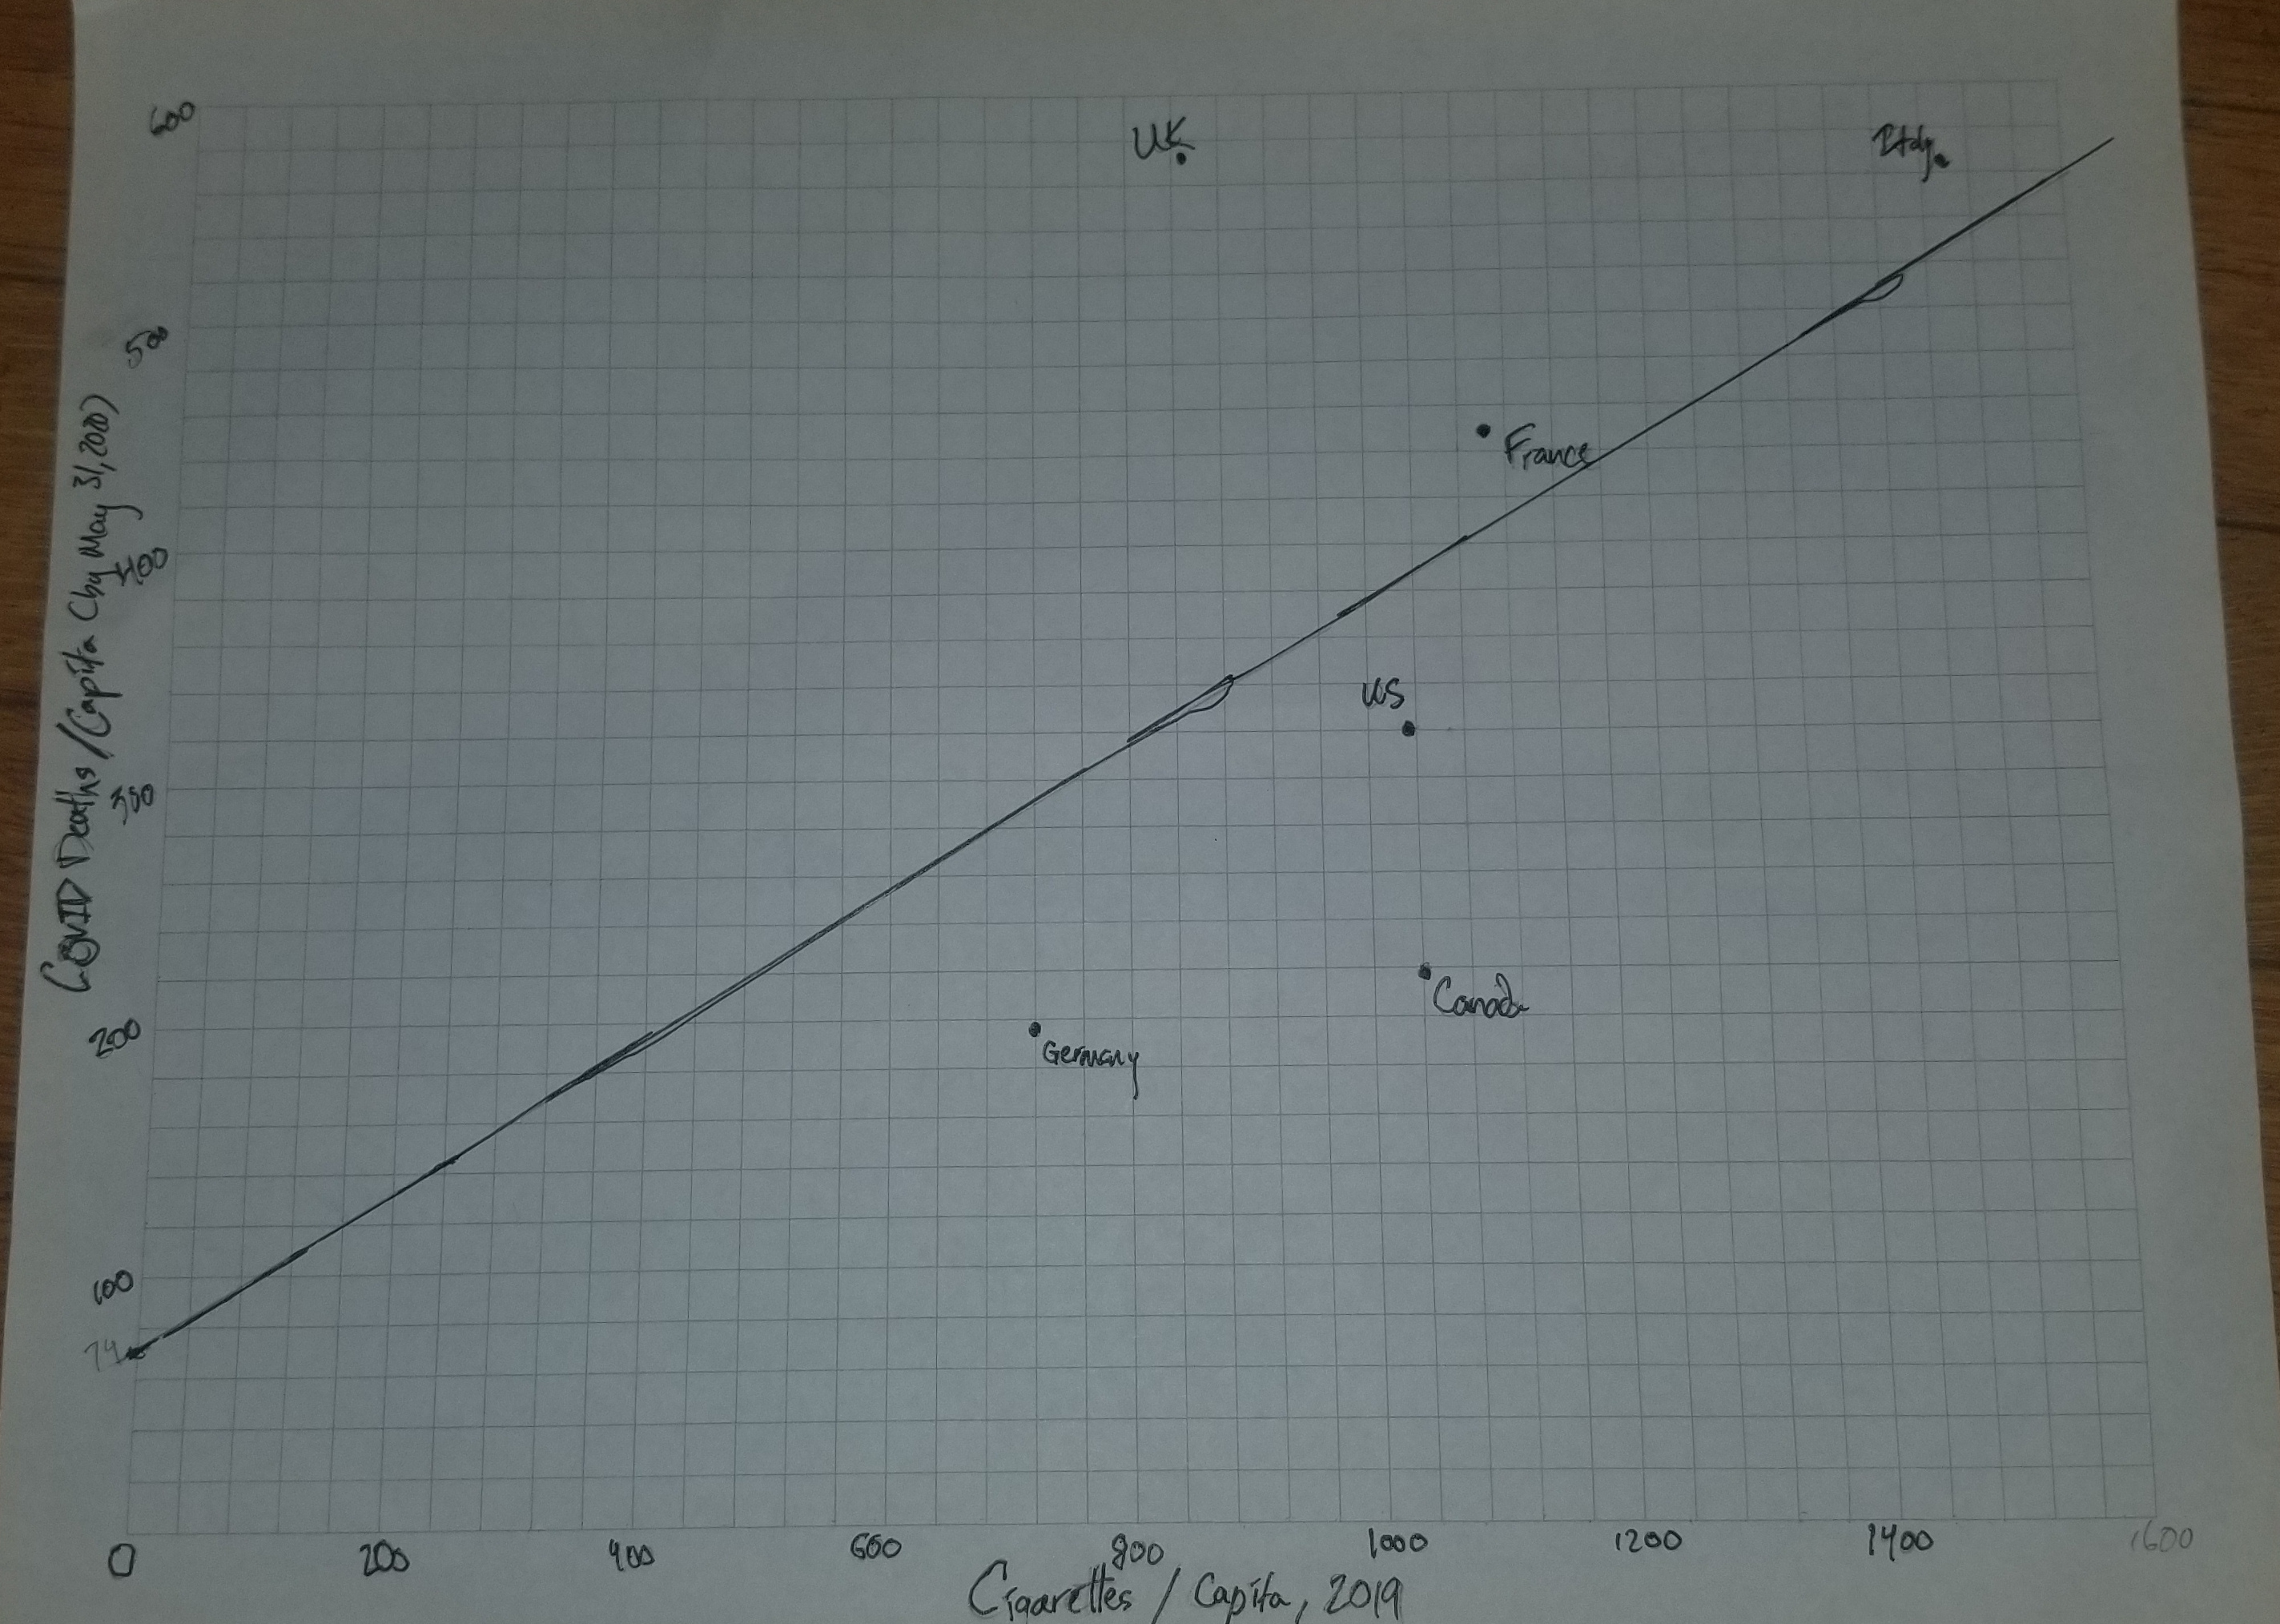
\includegraphics[width=\textwidth]{problem2.jpg}

\section*{Problem 3}
\subsection*{a}

Under the assumption that the population in a opposite-sex relationship has no significant difference between the wider male / female populations, the population mean is $\frac{1}{2}(\mu_M + \mu_W)$, as each relationship has a man and a woman in this case, so we want $E\left[\frac{1}{2}(M + W)\right] = \frac{1}{2}(\mu_M + \mu_W)$ where $M, W$ are the height distributions for men and women respectively.

\subsection*{b}

In particular, simple random sampling yields that $E[M_1] = E[M_2] = \mu_M$ and $E[W_1] = E[W_2] = \mu_W$. Then, since expectation is linear, we have
\begin{align*}
  E[\overline{H}] &= E\left[\frac{1}{4}(M_1 + M_2 + W_1 + W_2\right] \\
                  &= \frac{1}{4}(E[M_1] + E[M_2] + E[W_1] + E[W_1]) \\
                  &= \frac{1}{4}(2\mu_M + 2\mu_W) = \frac{\mu_M + \mu_W}{2}
\end{align*}
which was what we wanted.

\subsection*{c}

I did this problem set backwards, so I show that $\Var(X + Y) = \Var(X) + \Var(Y) + 2\Cov(X,Y)$ in problem 5. In general, we can use this
% \begin{align*}
%   \Cov(X + Y, W + Z)  =& E[(X+Y)(W+Z)] - E[X+Y]E[W+Z]                                              \\
%                       =& E[XW + XZ + YW + YZ] - (E[X] + E[Y])(E[W] + E[Z])                         \\
%                       =& E[XW] + E[XZ] + E[YW] + E[YZ] \\
%                        & - E[X]E[W] - E[X]E[Z] - E[Y]E[W] - E[Y]E[Z] \\
%                       =& \Cov(X,W) + \Cov(X,Z) + \Cov(Y,W) + \Cov(Y,Z)
% \end{align*}
to see that
\[
  \Var\left(\sum_{i=1}^nX_i\right) = \sum_{i=1}^n\Var(X_i) + \sum_{i,j=1,j\neq i}^n\Cov(X_i, X_j)
\]

In particular, we have shown it for $n = 2,$ but if it holds for $n = k$, we have that

\begin{align*}
  \Var\left(\sum_{i=1}^{k+1}X_i\right) &= \Var\left(\sum_{i=1}^kX_i\right) + \Var(X_{k+1}) + 2\Cov\left(\sum_{i=1}^{k+1}X_i, X_{k+1}\right) \\
                                       &= \sum_{i=1}^{k+1}\Var(X_i) + \sum_{i,j=1,i\neq q}^{k+1} \Cov(X_{i},X_{j})
\end{align*}

% In this specific case of four variables, we have that
% \begin{align*}
%   \Var(X_{1} + X_{2} + X_{3} + X_{4}) &= \Cov(X_{1} + X_{2} + X_{3} + X_{4}, X_{1} + X_{2} + X_{3} + X_{4}) \\
%                       &= \Cov(X_{1} + X_{2}, X_{3} + X_{4}) + \Cov()
% \end{align*}

In this problem, we have that the only nonzero covariances are $\Cov(M_1, W_1) = \Cov(M_2, W_2) = 0.5$, such that we have
\begin{align*}
  \Var(\overline{H}) & = \Var\left( \frac{1}{4}(M_{1} + M_{2} + W_{1} + W_{2})\right)                                            \\
                     & = \frac{1}{16}\Var(M_{1} + M_{2} + W_{1} + W_{2})                                                         \\
                     & = \frac{1}{16}(\Var(M_{1}) + \Var(M_{2}) + \Var(W_{1}) + \Var(W_{2}) + 2\Cov(M_1, W_1) + 2\Cov(M_2, W_2)) \\
                     & = \frac{1}{16}(\sigma^{2}_{M} + \sigma^{2}_{W} + 2(0.5) + 2(0.5)) \\
                     & = \frac{1}{16}(\sigma^{2}_{M} + \sigma^{2}_{W} + 2) \\
\end{align*}

\subsection*{d}

Since all covariances are 0, we have that analagously to the last part,
\begin{align*}
  \Var{\widetilde{H}} &= \Var(\gamma_{M}M_{1} + \gamma_{M}M_{2} + \gamma_{W}W_{1} + \gamma_{W}W_{2}) \\
                     &= \gamma_{M}^{2}\Var(M_{1}) +  \gamma_{M}^{2}\Var(M_{2}) +  \gamma_{W}^{2}\Var(W_{1}) +  \gamma_{W}^{2}\Var(W_{2}) \\
                     &= 2\gamma_{M}^{2}\sigma_{M}^{2} + 2\gamma_{W}^{2}\sigma_{W}^{2} \\
\end{align*}

Its easy to see that this function is twice differentiable with positive-definite Hessian (as we have that $\frac{\partial^{2} f}{\partial \gamma_{M}^{2}} = 4\sigma_{M}^{2} > 0$, and $\frac{\partial^{2} f}{\partial \gamma_{M}\partial \gamma_{W}} = 0$, so all pivots of the Hessian are positive), so it is convex.

Since we want the minimal variance under the condition $2\gamma_{M} + 2\gamma_{W} = 1$, we have that we need
\[
  \mathcal{L}(\gamma_{M}, \gamma_{Y}, \lambda) = 2\gamma_{M}^{2}\sigma_{M}^{2} + 2\gamma_{W}^{2}\sigma_{W}^{2} - \lambda(2\gamma_{M} + 2\gamma_{W} - 1)
\]
has vanishing partials. Then,
\begin{align*}
  \frac{\partial \mathcal{L}}{\partial \gamma_{M}} & = 4\gamma_{M}\sigma_{M}^{2} - 2\lambda = 0        \\
  \frac{\partial \mathcal{L}}{\partial \gamma_{Y}} & = 4\gamma_{W}\sigma_{W}^{2} - 2\lambda = 0        \\
  \intertext{This gives that}
  \gamma_{M}                                       & = \frac{\sigma_{W}^{2}}{\sigma_{M}^{2}}\gamma_{W} \\
  \intertext{Considering the last partial, we have that}
  \frac{\partial \mathcal{L}}{\partial \lambda}    & = -2\gamma_{M} - 2\gamma_{W} + 1 = 0              \\
                                                   & = -2(\frac{\sigma_{W}^{2}}{\sigma_{M}^{2}}\gamma_{W} + \gamma_{W}) + 1 \\
                                                   & = -2\frac{\sigma_{W}^{2} + \sigma_{M}^{2}}{\sigma_{M}^{2}}\gamma_{W} + 1 \\
  \intertext{Which gives that}
  \gamma_{W} &= \frac{\sigma_{M}^{2}}{2(\sigma_{M}^{2} + \sigma_{W}^{2})} \\
  \gamma_{M} &= \frac{\sigma_{W}^{2}}{2(\sigma_{M}^{2} + \sigma_{W}^{2})} \\
\end{align*}
are the coefficents such that $\widetilde{H} = \gamma_{M}M_{1} + \gamma_{M}M_{2} + \gamma_{W}W_{1} + \gamma_{W}W_{2}$ has a minimal sample variance (since we know that the function is convex, we know this is a minimum).

\section*{Problem 4}

\subsection*{a}

We have the hypotheses:

\begin{align*}
  H_{0}&: \mu_{B} - \mu_{S} = 0 \\
  H_{1}&: \mu_{B} - \mu_{S} \neq 0\\
\end{align*}

where $\mu_{B}, \mu_{S}$ are the population averages of the height of males and females, respectively, at this age, and $H_{1}$ is the alternative hypothesis.

\subsection*{b}

An unbiased estimate of the difference between $\mu_{B}$ and $\mu_{S}$ by $\overline{Y_{Boys}} - \overline{Y_{Girls}}$.

In this particular sample, $\overline{Y_{Boys}} - \overline{Y_{Girls}} = 57.8 - 58.4 = -0.6$.

\subsection*{c}

The variance of the estimator, if we know the population variances $\sigma^{2}_{Boys}$ and $\sigma^{2}_{Girls}$, will be, as each sampling is assumed to be i.i.d, is
\begin{align*}
  \Var(\overline{Y_{Boys}} - \overline{Y_{Girls}}) &= \Var(\overline{Y_{Boys}}) + \Var(\overline{Y_{Girls}}) \\
                                                   &= \Var\left(\frac{1}{n_{Boys}}\sum_{i=1}^{n_{Boys}} Y_{Boys,i}\right) + \Var\left(\frac{1}{n_{Girls}}\sum_{i=1}^{n_{Girls}} Y_{Girls,i}\right) \\
                                                   &= \frac{1}{n_{Boys}^{2}}\Var\left(\sum_{i=1}^{n_{Boys}} Y_{Boys,i}\right) + \frac{1}{n_{Girls}^{2}}\Var\left(\sum_{i=1}^{n_{Girls}} Y_{Girls,i}\right) \\
  &= \frac{\sigma^{2}_{Boys}}{n_{Boys}} + \frac{\sigma^{2}_{Girls}}{n_{Girls}}
\end{align*}

Then, the variance of that estimator can be estimated; in particular, we know that the standard deviation of the sampling distribution is $s^{2}_{Boys} / n_{Boys}$ and $s^{2}_{{Girls}} / n_{{Girls}}$ for $\overline{Y_{Boys}}$ and $\overline{Y_{Girls}}$ respectively. Further, since we know that $\overline{Y_{Boys}}$ and $\overline{Y_{Girls}}$ are constructed from different randomly selected sample, they are independent, and thus we can estimate the variance of the earlier estimator to be $\frac{s^{2}_{{Boys}}}{n_{{Boys}}} + \frac{s^{2}_{{Girls}}}{n_{{Girls}}}$, as we know the sampling variance to be a consistent estimator for the population varinace.

This comes out to $0.765$ in this case.

\subsection*{d}

We have that $50 \approx \infty$, so by the law of large numbers we have that $\overline{Y_{Boys}}$ and $\overline{Y_{Girls}}$ are approximately normally distributed, so we have that the $t$-statistic can be given by
\[
  t = \frac{\overline{Y_{Boys}} - \overline{Y_{Girls}}}{\sqrt{\frac{s^{2}_{{Boys}}}{n_{{Boys}}} + \frac{s^{2}_{{Girls}}}{n_{{Girls}}}}}
\]

In particular, since we know that $\overline{Y_{Boys}} - \overline{Y_{Girls}}$ is approximately distributed with mean $\mu_{{Boys}} - \mu_{Girls}$ and variance $\sigma^{2}_{Boys} / n_{Boys} + \sigma^{2}_{Girls} / n_{Girls}$  where $\sigma^{2}_{X}$ are the population variances (as it is the difference of two approximately normal distributions), $\frac{\overline{Y_{Boys}} - \overline{Y_{Girls}} - (\mu_{{Boys}} - \mu_{Girls})}{\sqrt{\sigma^{2}_{Boys} / n_{Boys} + \sigma^{2}_{Girls} / n_{Girls}}}$ is then the standard normal distribution.

Assuming the null hypothesis, we would then have by the law of large numbers that $t$, for large $n_{Boys}, n_{Girls}$, is standard normally distributed itself, as $\mu_{Boys} - \mu_{Girls} \rightarrow 0$, and $\frac{s^{2}_{{Boys}}}{n_{{Boys}}} + \frac{s^{2}_{{Girls}}}{n_{{Girls}}} \rightarrow \sigma^{2}_{Boys} / n_{Boys} + \sigma^{2}_{Girls} / n_{Girls}$. (This isn't rigorous, but the result is true, and the justification is at least \textit{morally} true.)

\subsection*{e}

In this case, we have that $t = -0.784$. The critical value is, since we know that $t$ is approximately standard normal, $2.575$, or $\Phi^{-1}(0.995)$, as we need that the mass under the tails on either end of the distribution total to $0.01$. Thus, the difference is not significant.

Intuitively, if we had used a one-sided test, we would have allowed all the mass to come from one side instead of both, and as the critical value is the value such that the mass under the tails beyond the critical value is $0.01$, we would've shifted the critical value closer to the mean of the standard normal distribution, i.e. 0, and thus have lowered it. In particular, for a onesided test we would have used $\Phi^{-1}(0.99) = 2.32$.

\subsection*{f}

A 95\% confidence interval can be given by
\[
  (\overline{Y_{Boys}} - \overline{Y_{Girls}}) \pm 1.96 \sqrt{\frac{s^{2}_{{Boys}}}{n_{{Boys}}} + \frac{s^{2}_{{Girls}}}{n_{{Girls}}}} = -0.6 \pm 1.96(0.765) = (-2.10, 0.90)
\]

\section*{Problem 5}
\subsection*{a}

We have that expectation is linear, such that 
\[
  E[\overline{Y}] = E\left[ \frac{1}{4}(Y_1 + Y_2 + Y_3 + Y_4)\right] = \frac{1}{4}(E[Y_1] + E[Y_2] + E[Y_3] + E[Y_4]) = \frac{1}{4}(4\mu) = \mu
\]

The variance satisfies for $a, b$ constants, $X, Y$ some random variables, 
\begin{align*}
  \Var(a + bX) &= E[(a+bX)^2] - E[a+bX]^2 \\
               &= a^2 + 2abE[X] + b^2E[X^2] - (a + bE[X])^2 \\
               &= a^2 + 2abE[X] + b^2E[X^2] - a^2 - 2abE[X] - b^2E[X]^2 \\
               &= b^2(E[X^2] - E[X]^2) = b^2\Var(X) \\
  \Var(X+Y) &= E[(X+Y)^2] - E[X+Y]^2 \\
            &= E[X^2] + E[Y^2] + 2E[XY] - E[X]^2 - E[Y]^2 - 2E[X]E[Y] \\
            &= E[X^2] - E[X]^2 + E[Y^2] - E[Y]^2 + 2(E[XY] - E[X]E[Y]) \\
            &= \Var(X) + \Var(Y) + 2\Cov(X,Y) \\
            \intertext{If $X, Y$ are independent, such as in i.i.d variables, then $\Cov(X,Y) = 0$, and}
            &= \Var(X) + \Var(Y)
\end{align*}

Thus, 
\begin{align*}
  \Var(\overline{Y}) &= \Var\left(\frac{1}{4}(Y_1 + Y_2 + Y_3 + Y_4\right) \\
                     &= \frac{1}{16}(\Var(Y_1 + Y_2 + Y_3 + Y_4)) \\
                     &= \frac{1}{16}(4\sigma^2) \\
                     &= \frac{1}{4}\sigma^2
\end{align*}

\subsection*{b}

\begin{align*}
  E[\widetilde{Y}] &= E\left[\frac{1}{8}Y_1 + \frac{1}{8}Y_2 + \frac{1}{4} Y_3 + \frac{1}{2}Y_4\right] \\
                   &= \frac{1}{8}E[Y_1] + \frac{1}{8}E[Y_2] + \frac{1}{4}E[Y_3] + \frac{1}{2}E[Y_4] \\
                   &= \frac{1}{8}\mu + \frac{1}{8}\mu + \frac{1}{4}\mu + \frac{1}{2}\mu = \mu
\end{align*}
so $\widetilde{Y}$ is unbiased.

The variance is
\begin{align*}
  \Var(\widetilde{Y}) &= \Var\left(\frac{1}{8}Y_1 + \frac{1}{8}Y_2 + \frac{1}{4} Y_3 + \frac{1}{2}Y_4\right) \\
                     &= \frac{1}{64}\Var(Y_1) + \frac{1}{64}\Var(Y_2) + \frac{1}{16} \Var(Y_3) + \frac{1}{4}\Var(Y_4) \\
                     &= \frac{11}{32}\sigma^2
\end{align*}

\subsection*{c}

We have that both $\overline{Y}$ and $\widetilde{Y}$ are unbiased estimators, but $\widetilde{Y}$ has a higher variance (as $\frac{1}{4} < \frac{11}{32}$). In that sense, since we want to be less susceptible to unlucky sampling (in particular, on average, $\widetilde{Y}$ is further from the true mean than $\overline{Y}$), we want to use $\overline{Y}$ over $\widetilde{Y}$. 

\subsection*{d}

A feature of the normal distribution is that two normally distributed variables $X, Y$ (which are independent) have that $Z = X + Y$ is also normally distributed with $E[Z] = E[X + Y]$ and $\Var(Z) = \Var(X) + \Var(Y)$. In particular, we also have that each of $aY_i$ is normal with $E[aY_i] = a\mu$ and variance $\Var(aY_i) = a^2\sigma^2$.

Then, this tells us that $\overline{Y}$ and $\widetilde{Y}$, as the sums of normally distributed independent variables, are both normally distributed themselves. The variances and expectations remain unchanged from earlier, with $E[\overline{Y}] = E[\widetilde{Y}] = \mu = 5$ and $E[\overline{Y}] = \frac{1}{4}\sigma^2 = \frac{3}{4}$ and $E[\widetilde{Y}] = \frac{11}{32}\sigma^2 = \frac{33}{32}$.

\section*{Problem 6}
\subsection*{a}

\[
  E[GPA \mid SAT = 1600] = 0.9 + 0.001(1600) = 0.9 + 1.6 = 2.5
\]

\subsection*{b}

\[
  E[GPA \mid SAT = 2200] = 0.9 + 0.001(2200) = 0.9 + 2.2 = 3.1
\]

\subsection*{c}

The law of total expectation and the linearity of expectation gives
\[
  E[GPA] = E[E[GPA \mid SAT]] = E[0.9 + 0.001SAT] = 0.9 + 0.001E[SAT] = 0.9 + 0.001(2000) = 2.9
\]

\section*{Problem 7}
\subsection*{a}

The law of total expectation gives us that
\[
  E[u] = E[E[u \mid X]] = E[0] = 0, E[u^2] = E[E[u^2 \mid X]] = E[\sigma^2] = \sigma^2
\]

This gives that the mean of $u$ is $E[u] = 0$ and the variance is $E[(u - E[u])^2] = E[u^2] - E[u]^2 = \sigma^2 - 0 = \sigma^2$.

\subsection*{b}

The covariance vanishes if we have that $E[u \mid X] = E[u]$:
\begin{align*}
  \Cov(u, X) &= E[(u - E[u])(X - E[X])] \\
  \intertext{Via linearity of expectation,}
             &= E[uX] - E[u]E[X] \\
  \intertext{Via law of total expectation,}
             &= E[E[uX \mid X]] - E[u]E[X] \\
  \intertext{Since $X$ is a constant when conditioned on itself,}
             &= E[XE[u \mid X]] - E[u]E[X] \\
             \intertext{We showed earlier that $E[u] = E[u \mid X] = 0$}
             &= E[XE[u]] - E[u]E[X] \\
             &= E[X]E[u] - E[u]E[X] \\
             &= 0
\end{align*}

In particular, this only relies on $E[u \mid X] = k$ for some constant, not necessarily 0.

\end{document}
% LocalWords:  NetID fancyplain LocalWords colorlinks linkcolor linkbordercolor
